\documentclass[acmtog]{acmart}
\usepackage{graphicx}
\usepackage{subfigure}
% Title portion
\title{Assignment 2 : Create A B-spline Surface} 
\author{Name:\quad Zhang Zhanrui  \\ student number:\quad 2019533227
	\\email:\quad zhangzhr2@shanghaitech.edu.cn}

% Document starts
\begin{document}
\maketitle

\vspace*{2 ex}


\section{Introduction}
In this assignment, A B-spline surface is created based on the given control point by using de Boor's algorithm. Then it is rendered with VAO and VBO in OpenGL.

Meanwhile, NURBS surface evaluation is supported. To demonstrate that, a group of custom control points with weight are used to render a sphere.

At last, a check box texture provided by TA is applied to all objects rendered.

\section{Implementation Details}
\subsection{de Boor algorithm for B-spline curve}
To evaluate a B-spline curve, a serious of control point, a knots vector, and degree. The curve can be interpreted as a combination of control points with a basis function as the coefficient. However, due to the local property, many control points don't contribute to a certain point, which make it a waste of time to evaluate all basis function and then add them together. Instead, de Boor's algorithm uses a recursive method to evaluate the point on the curve.

First, a knot vector divides the parameter space into different intervals, telling us how a curve is divided into many section. A function named `insertNum()' is defined to find which interval the parameter given is in. Let the parameter $t$ is in the $k^{\mathrm{th}}$ interval. Then `degree+1' control points starting from $k$ are added to a intermediate vector.
We interpolate between each pair of successive control points to get a new intermediate control point, after `degree' times of iteration, we can find the coordinate of the final point on the B-spline curve.

\subsection{Calculate the position of a point on a B-spline surface}
Now we can extend the evaluation for curve to surface. If $n\times m$ control points are provided, and point with coordinate $(u,v)$ in parameter space is to be evaluated, we need to fix $v$ first and calculate one point for each row of the $m$ control points. Then we uses the newly generated $n$ points as the new control points for $u$ direction, and apply de Boor algorithm again, we and calculate the coordinate in world space of point $(u, v)$.

\subsection{Calculate the normal vector of the B-spline surface}
To render a 3D surface, a normal vector is needed. When evaluate a B-spline curve by de Boor's algorithm, it is very easy to get the tangent vector of a point, just by recording the last two intermediate control point and subtracting one from the other. By evaluating B-spline surface twice, each time starting from a different direction, it is easy to get the tangent vector in both $u$ and $v$ direction. Then normal vector is just the cross product of those two tangent vectors.

\subsection{Render a surface with VAO and VBO}
To render a whole surface, two loops are needed to iterate through all $u$ and $v$ with a sample step. After those two loops, a series of sample point are generated. Here, for simplicity, the sample step are uniformed and remains constant. In addition, a simple triangulation process is required to get the face index to render the mesh. We just divide each grid on $u-v$ space into two triangles and put the index of vertices into  the faceIndex vector. The index of lines are created similarly. Now we can send them into the OpenGL rendering pipeline and render them. The shader used is the same as in assignment 1.

\subsection{Apply texture on the surface}
To apply texture on the surface of, a $(u, v)$ coordinate is needed. In out cases, we just set the $(u,v)$ coordinate in parameter space as the coordinate of texture.

In detailed implementation, A class named `Texture' is constructed. It will load the texture image by using `stb\_image.h'. Then it will set the correct way to wrap the texture and generate mipmap. Then when calling `draw()' method in SurfaceRender class, the texture generated will be binded to corresponding object.

\subsection{Implement NURBS}
de Boor algorithm also works for the NURBS surface, with a little adjustment. NURBS surface requires one more dimension, which is the weight of each control point. In the code, we just need to change corresponding `glm::vec3' variable to `glm::vec4' type. The new control point in 4-dimensional space will be $(x\cdot w, y\cdot w, z\cdot w, w)$, where $x$, $y$ and $z$ are original 3-D coordinate and $w$ the weight.

After applying de Boor algorithm on a series of 4-D control points, we can get a 4-D coordinate. Then by dividing the $x$, $y$ and $z$ with $w$, the 4-D point can be projected back to 3-D space.


In this assignment, to showcase the unique property of NURBS surface, a series of control points (with weight) are specified in the header files, `nurbs\_data.h'.

To render the normal control point without weight, we just need to assign a uniformed weight $w = 1$ to every control point.

\section{Results}
The result of this assignment are as follow. You can control the camera view by pressing A, S, D, W and moving the camera. You can press key `1', `2' or `3' to switch between B-spline surface (line mode), B-spline surface (solid surface) and NURBS surface (sphere).


\subsection{The B-spline surface with texture}
The rendering results of B-spline surface are shown in the following picture.

As can be seen in the picture, for the given control point, the sampled point close to edge are sparser, while the point close to the center are more dense.

\begin{figure}[h]
	\centering
	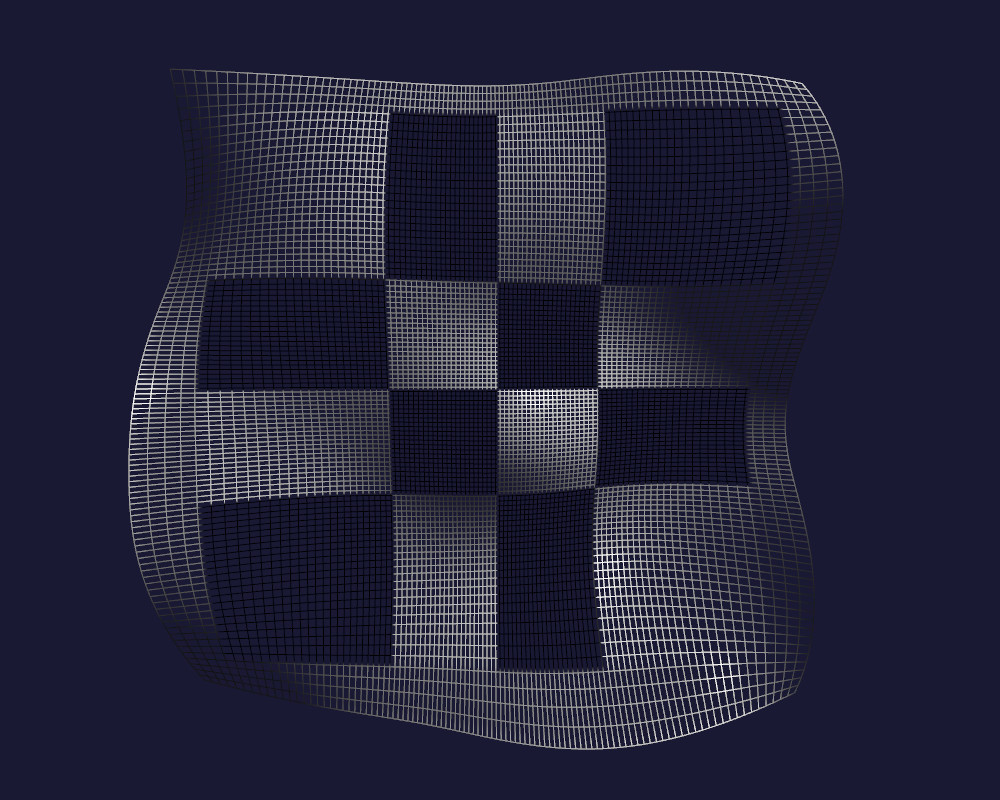
\includegraphics[scale=0.25]{line.png}
	\caption{B-spline surface with texture (drawn in line)}
\end{figure}


\begin{figure}[h]
	\centering
	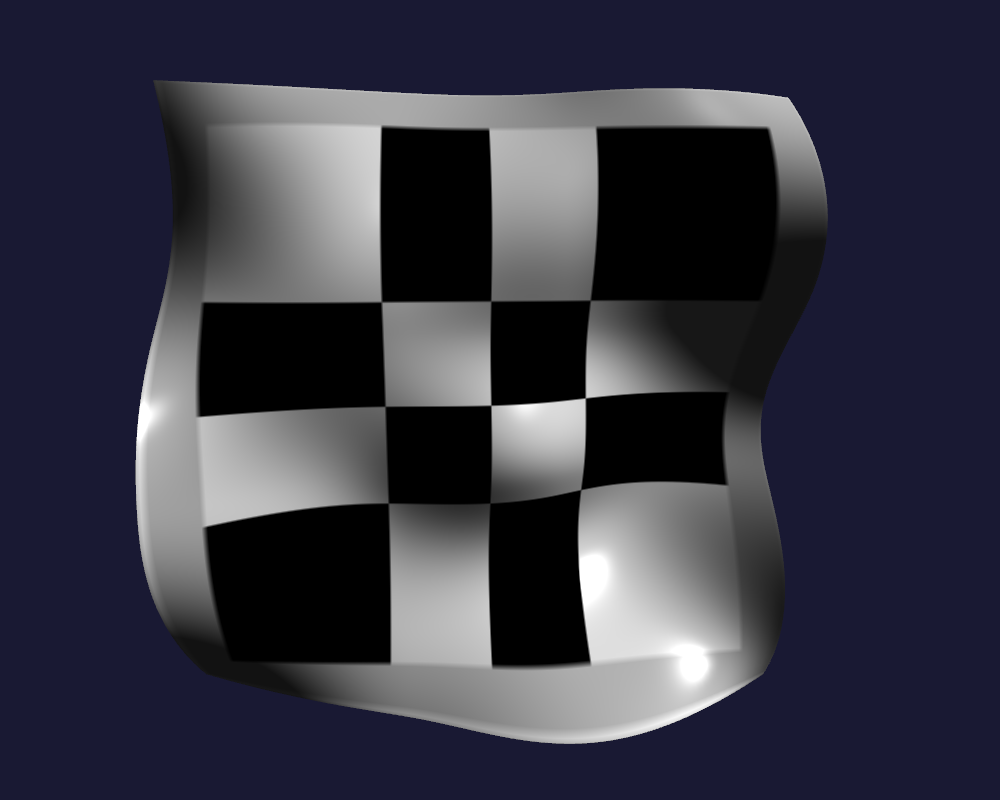
\includegraphics[scale=0.25]{mesh.png}
	\caption{B-spline surface with texture}
\end{figure}

\subsection{NURBS surface}
A sphere is rendered and the result is shown in the following picture.
\begin{figure}[h]
	\centering
	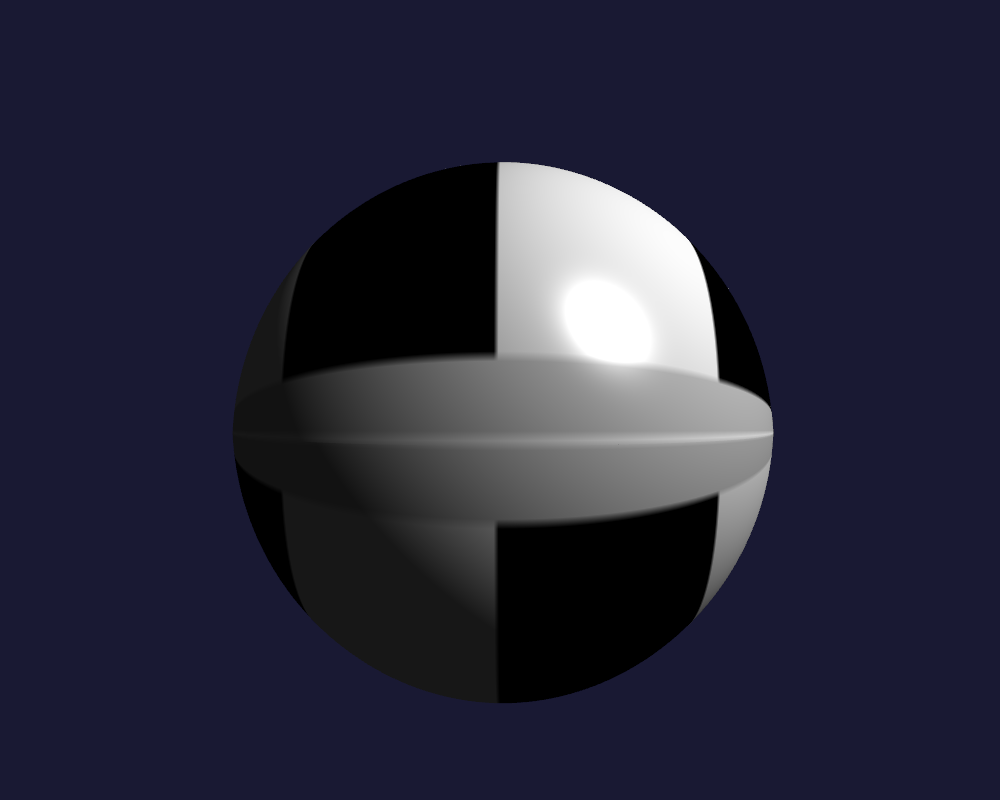
\includegraphics[scale=0.25]{nurbs.png}
	\caption{NURBS Sphere}
\end{figure}

\end{document}
